\documentclass[a4paper, 12pt]{scrartcl}
\usepackage[ngerman]{babel}
\usepackage[utf8]{inputenc}
\usepackage[T1]{fontenc}
\usepackage{minted}
\usepackage{graphicx}
\usepackage{hyperref}
\usepackage{lscape}
\usepackage{amsmath}
\title{Dokumentation zum Beleg für Rechnernetze I}
\author{Philipp Wenskus - s72902}

\begin{document}
\newminted{java}{linenos,frame=lines}

\maketitle
\newpage
\tableofcontents
\newpage
\section{Belegaufgabe}
Die Aufgabe des Belegs besteht darin, zwei Programme (Client + Server) in Java zu erstellen, bei dem der Client eine beliebige Datei sendet und der Server diese empfängt. Als Grundlage für die Übertragung soll das UDP-Protokoll genutzt werden, welches in Java als vorgefertigte Funktion zu Verfügung steht.\\
Ein Startpaket am Anfang der Übertragung liefert dem Server nötige Informationen zu der Datei die vom Client empfangen wird. Die Datei selbst soll vom Client in kleinere Pakete aufgeteilt werden. Beim Übertragen des letzten Datenpakets muss die Prüfsumme(CRC32) der Datei mitgesendet werden welche der Server dann überprüft um die Datei zu verifizieren. Um Fehler in der Übertragung der einzelnen Pakete zu erkennen und diese ggf. auszubessern sollte ein Stop-And-Wait Protokoll implementiert werden bei dem der Server erfolgreich empfangene Pakete mit einen Acknowledgement(kurz Ack), welches er an Client sendet, bestätigt.

\section{Stop-And-Wait Protokoll} \label{stopNwait}
Um das Programm besser zu verstehen wird hier die Funktionsweise und der Ablauf des Stop-And-Wait Protokolls beschrieben.
\subsection{Ablauf}
\begin{figure}[h] 
  \centering
     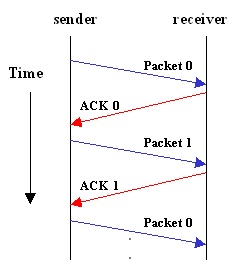
\includegraphics[scale=1.2]{e-stop.jpg}
  \caption{Übertragung mit dem Stop-And-Wait Protokoll, Quelle: \href{http://www.isi.edu/nsnam/DIRECTED_RESEARCH/DR_HYUNAH/D-Research/e-stop.gif}{www.isi.edu}}

  \label{stop_n_wait}
\end{figure}
\begin{enumerate}
	\item 	Der Client sendet sein vorher zusammengestelltes Paket an den Server
	\item 	Der Server empfängt das Paket erfolgreich und sendet ein Acknowledgement(hier Sessionnr. und Paketnr.) an den Client 
	\item 	Der Client empfängt das Ack, überprüft dies und sendet, falls vorhanden, das nächste Paket
\end{enumerate}
\subsection{Probleme und Fehlerbekämpfung bei der Übertragung}
Der oben beschriebene Ablauf stimmt nur, wenn die Übertragung fehlerfrei funktioniert. Da dies nicht immer gewährleistet werden kann, sind im Protokoll mehrere Kontrollmechanismen, welche Fehler erkennen und ausbessern sollen.\\
Folgende zwei Szenarien sind möglich welche man auch in Abbildung \ref{stop_n_wait_fail} sehen kann
\begin{enumerate}
\item Paket kommt nicht beim Server an (Abbildung \ref{stop_n_wait_fail}, rechte Seite)
\begin{itemize}
\item Der Client sendet ein Paket an den Server. Der Server empfängt das Paket nicht und sendet somit kein Ack. Der im Client eingestellte \textit{Timeout} für das Empfangen des Acks läuft ab. Ist der Timeout abgelaufen sendet der Client das Paket erneut (hier bis zu 10 mal). Sobald der Server das Paket erfolgreich empfangen hat schickt er das Ack zum Client.
\end{itemize}
\item Acknowledgement kommt nicht beim Client an (Abbildung \ref{stop_n_wait_fail}, linke Seite)
\begin{itemize}
\item Der Client sendet ein Paket an den Server. Der Server empfängt das Paket erfolgreich und schickt ein Ack an den Client. Der Client bekommt das Ack nicht, wodurch der \textit{Timeout} in Kraft tritt und der Client die Datei nochmals sendet (hier bis zu 10 mal). Der Server empfängt das Paket erneut, verwirft es und schickt nochmals das Ack an den Client. 
\end{itemize}
\end{enumerate}
\begin{figure}[htbp] 
  \centering
     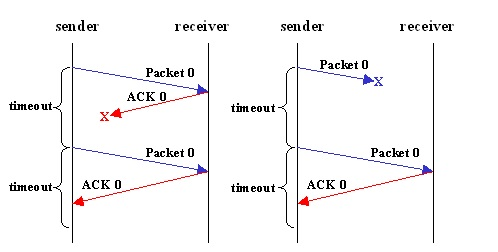
\includegraphics[width=0.8\textwidth]{e-stop1.jpg}
  \caption{Fehlerszenarien des Stop-And-Wait-Protokolls, Quelle: \href{http://www.isi.edu/nsnam/DIRECTED_RESEARCH/DR_HYUNAH/D-Research/e-stop1.gif}{www.isi.edu}}

  \label{stop_n_wait_fail}
\end{figure}
\newpage
\section{Funktionsweise}
In Folgenden werden die beiden Programme und deren Funktionen detaillierter beschrieben.
\subsection{Client} \label{Client}
Der Client ist für das Senden einer Datei zum Empfänger zuständig. Dabei splittet der Client die Datei in mehrere kleine Pakete auf und verschickt diese dann. Um den Server auf die eingehende Datei vorzubereiten schickt der Client ein Startpaket mit allen nötigen Informationen an den Empfänger.
\subsubsection{Startpaket} \label{Startpaket}
Das Startpaket wird am Anfang der Verbindung an den Server gesendet um diesen eine neue Verbindung zu signalisieren und nötige Informationen zu liefern. Nachfolgend wird auf die einzelnen Bestandteile des Startpakets genauer eingegangen. 
\begin{figure}[h]
	\centering
		\begin{tabular}{|l|}
		\hline		
		\multicolumn{1}{|c|}{Startpaket}\\
		\hline \hline
		- Sessionnr. (2 Byte)\\
		- Paketnr.   (1 Byte, im Startpaket immer 0)\\
		- Kennung 'Start' (5 Byte, ASCII)\\
		- Dateigröße (8 Byte)\\
		- Länge des Dateinamens (2 Byte)\\
		- Dateiname (0-255 Byte, UTF-8)\\
		- CRC32 über gesamtes Startpaket (4 Byte)\\
		\hline
		\end{tabular}
\end{figure}
\paragraph{Sessionnummer}
Die Sessionnr. ist eine zufällig generierte, 2 Byte große positive Zahl welche durch die Random-Funktion von Java erzeugt wird:
\begin{javacode} 
public static short randomSession()
{
	Random randSession = new Random();
	    	
	short randomNumber = (short)randSession.nextInt(Short.MAX_VALUE + 1);
	return randomNumber;
}
\end{javacode}
\textit{Short.MAX\_VALUE} gibt dabei die möglichst große Positive Zahl eines einer Short-Variable an. Die +1 steht dabei für die Null, die noch nicht in Short.MAX\_VALUE enthalten ist.
\paragraph{Paketnummer}
Die Paketnummer ist im Startpaket immer 0 und kann in den folgenden Paketen entweder 1 oder 0 annehmen (Packetnr mod(2))
\begin{javacode}
int i = 0; //Globale Variable der Client-Klasse

public static byte[] getnewPackageNr()
{
	byte[] packageNr = new byte[1]; 
	packageNr[0] = (byte)(i%2);
	Client.i++;
	return packageNr;	
}
\end{javacode}
Die Funktion \textit{getnewPackageNr} gibt die Paketnummer für das kommende Paket zurück. Die globale Variable i, die in der Funktion modulo 2 gerechnet wird, ist die dabei die echte Paketnummer (z.B. für das Startpaket gleich 0 $\Rightarrow$ 0 mod(2) = 0)

\paragraph{Kennung}
Die Kennung ist ein weiteres Merkmal an dem der Server das Startpaket erkennen soll. Sie ist immer 'Start' und als ASCII formatiert. 

\paragraph{Dateigröße}
Der Server benötigt die Dateigröße um festzustellen wann die Daten der Datei vollständig angekommen sind um dann am Ende des letzten Datenpakets den CRC-Code der Datei auszulesen zu können
\begin{javacode}
File file = new File(filepathString);
//Dateilänge (64 Bit = 8 Byte)
byte[] filelength = ByteBuffer.allocate(8).putLong(file.length()).array();
\end{javacode}
\paragraph{Dateinamenlänge}
Der Empfänger braucht die Dateilänge für das Auslesen des Dateinamens aus dem Startpaket, da dieser Teil eine variable Größe hat.
\begin{javacode}
File file = new File(filepathString);
....
String filenameString = file.getName(); 
short filenamelengthShort = (short)filenameString.length();
byte[] filenamelength = 
		ByteBuffer.allocate(2).putShort(filenamelengthShort).array();
\end{javacode}
\textit{filenamestring} ist hier der Dateiname der zu sendenden Datei, \textit{filenamelengthshort} die Länge des Namens. 
\paragraph{Dateiname}
Übergibt den Namen der Datei, UTF-8 formatiert, an den Server. Dieser Speichert die Datei unter dem gleichen Namen ab (bei schon vorhanden Dateinamen $\Rightarrow$ Dateiname + 1)
\begin{javacode}
File file = new File(filepathString);
....
String filenameString = file.getName(); 
short filenamelengthShort = (short)filenameString.length();
//Dateiname als UTF8 String (0-255 Byte) -> länge kann von filenamelength abhängig gemacht werden
byte[] filename = new byte[filenamelengthShort];
filename = filenameString.getBytes("UTF-8");
\end{javacode}
\paragraph{CRC32 (Startpaket)}
Sobald alle Daten des Startpakets vorbereitet sind werden diese über einen ByteBuffer in ein Bytearray geschoben um die Prüfsumme für das Startpaket zu berechnen.
\begin{javacode}
Checksum checksumStart = new CRC32();
checksumStart.update(startPackage_withoutCRC.array(), 
	0, startPackage_withoutCRC.array().length);
long crcStartNumber= checksumStart.getValue();
byte[] crcStart = longtoByteCRC(crcStartNumber);
	    	
/*Startpaket mit CRC-Code zusammenfügen*/
ByteBuffer startPackageBuff = ByteBuffer.allocate
		(startPackage_withoutCRC.array().length + crcStart.length);
//Add CRC Code 
startPackageBuff.put(startPackage_withoutCRC.array());
startPackageBuff.put(crcStart);
byte[] startPackage = startPackageBuff.array();
\end{javacode}
Sobald die Prüfsumme berechnet wurde wird sie an das Startpaket angefügt, welches somit versendet werden kann.
Problem dabei ist, den CRC-Code, welcher von der Java-Funktion als \textit{long} zurückgegeben wird in ein 4-Byte-Aaray zu schreiben.
Dieses Problem löst die hier verwendete Funktion longtoByteCRC:
\begin{javacode}
public static byte[] longtoByteCRC(long checksum)
{
	byte[] checksumBytes=new byte[4];
	for(int j=4-1;j>=0;j--) 
	{
		for(int i=0;i<8;i++) 
		{
			if((checksum%2)==1) {
				checksumBytes[j] |=(1 << i);
			} else {
				checksumBytes[j] |=(0 << i);
			}
			checksum=checksum/2;
		}
	}
	return checksumBytes;
}
\end{javacode}
Durch Bitoperationen werden die Bytes des errechneten \textit{long} Wertes, in ein 4-Byte-Array konvertiert.
\subsubsection{Datenpakete} \label{Datenpakete}
Die Datenpakete werden gesendet sobald das Startpaket erfolgreich gesendet wurde. Sie enthalten die Sessionnr. (die gleiche wie das Startpaket) eine Paketnummer (abwechselnd 0 oder 1) und die Daten der Datei, die vom Client gesplittet wurde. Außerdem enthält das letzte Datenpaket den CRC Code der gesendeten Datei um diese zu verifizieren.
\begin{figure}[h]
	\centering
		\begin{tabular}{|l|}
		\hline		
		\multicolumn{1}{|c|}{Datenpaket}\\
		\hline \hline
		- Sessionnr. (2 Byte, gleiche wie im Startpaket)\\
		- Paketnr.   (1 Byte, 0 oder 1)\\
		- Daten\\
		- CRC32 der Datei (4 Byte, nur im letzten Paket)\\
		\hline
		\end{tabular}
\end{figure}
\subsubsection{Start des Clients}
Zum Start des Clients müssen Adresse des Empfängers, der Port mit dem dieser Daten empfängt und der Pfad der Datei die gesendet werden soll, angegeben werden. Um den Client einfacher zu starten wird er über ein Script aufgerufen:
\begin{center}
./client-udp <Server Adresse> <Port> <Dateiname/Dateipfad>
\end{center}   
Sollten zu wenig Parameter übergeben worden sein wird der Client nicht gestartet.
\subsubsection{Programmablauf des Clients}
Nach dem Starten mit den erforderlichen Parametern wird das unter \ref{Startpaket} angegebene Paket erstellt. Das Zusammenstellen des Paketes übernimmt die Funktion \textit{getStartPackage}, welche die Datei und die zuvor generierte Sessionnr. übergeben bekommt, und das fertige Byte-Array mit den Daten des Startpaketes zurückgibt. Danach wird das Startpaket an dem Server übermittelt. Dies geschieht über das UDP-Socket (DatagramSocket).
\begin{javacode}
DatagramSocket socket = new DatagramSocket();   //öffne den UDP-Socket
socket.setSoTimeout(TIMEOUT);					

InetAddress serverAddress = InetAddress.getByName(host);
DatagramPacket startPackage = 
	           new DatagramPacket(startPackageByte, startPackageByte.length, serverAddress, port);
	        
long timeStart = System.nanoTime();	//starte Zeitabnahme
socket.send(startPackage);
\end{javacode}
Der Timeout wird hier auf einen Anfangswert festgelegt und während des Sendens je nach Verbindung entweder erhöht oder verringert.
Da sich über ein DatagramSocket nur ein DatagramPacket versendet lässt, wird ein DatagramPacket erstellt, dass die Daten des Pakets, die Länge der Daten, die Adresse des Empfängers und den Port den der Empfänger benutzt enthält.\\
Nun ist der Ablauf wie im Kapitel \ref{stopNwait} beschriebenen Stop-And-Wait Protokoll.\\
Der Client wartet auf das Ack(siehe \ref{ACK}). Sollte er das Paket empfangen überprüft er ob die Paket- und Sessionnr. mit dem gesendeten Paket übereinstimmen. Ist das der Fall setzt der Client mit dem Senden der Datenpakete fort. Wenn ein Timeout beim Empfangen eintritt oder das Ack fehlerhaft ist wird das Startpaket bis zu 10 mal erneut gesendet. Sollte dann immer noch kein richtiges Ack angekommen sein wird eine Fehlermeldung ausgegeben und der Client beendet.
\\\\
Zum übertragen der Datei wird immer ein Stück der Datei in einen Bytebuffer geschrieben. Dann wird das unter Kapitel \ref{Datenpakete} beschriebene Datenpaket erstellt und an den Server gesendet. Es wird wie auch beim Startpaket auf das Ack gewartet. Sollte dies erfolgreich ankommen wird das Einlesen, Senden und Empfangen in einer while-Schleife so lange wiederholt, bis die Datei ganz eingelesen wurde.  

\begin{javacode}
FileInputStream fileStream = new FileInputStream(file);
FileChannel fileChnl = fileStream.getChannel();
ByteBuffer filebuffer = ByteBuffer.allocate(PACKAGESIZE); 
while(fileChnl.read(filebuffer) > 0)
{
	long current;
	DatagramPacket dataPackage;
	filebuffer.flip();
	sendedBytes += PACKAGESIZE;
	if (sendedBytes < file.length())
	{
		byte[]dataPackageBytes = getDataPackage(filebuffer.array(), sessionNr);
		dataPackage = 
			new DatagramPacket(dataPackageBytes, dataPackageBytes.length, serverAddress, port);
		current = dataPackageBytes.length;
		timeStart = System.nanoTime();
		socket.send(dataPackage);
		filebuffer.clear();
	}
	/******Falls letztes Paket gesendent wird*****/
	else
	{
		socket.setSoTimeout(1500); //Timeout wird erhöht da berechnen von CRC Code im Server länger dauern kann (bei großen Dateien)
		int restBytes = (int)(PACKAGESIZE -(sendedBytes-filesize));
		byte[]dataPackageBytes = 
			getDataEndPackage(filebuffer.array(), 
			sessionNr, checksumFile, restBytes);
		dataPackage = 
			new DatagramPacket(dataPackageBytes, 
			dataPackageBytes.length,serverAddress, port);
		current = dataPackageBytes.length;
		timeStart = System.nanoTime();
		socket.send(dataPackage);
		filebuffer.clear();
	}
	.....
}
\end{javacode} 
Sollte das letzte Paket gesendet werden wird der else-Zweig des Codes ausgeführt, der neben den Daten noch den CRC-Code der Datei an das Datenpaket anfügt.\\
Wenn der Client alle Pakete an den Server geschickt hat und ein Ack erhält ist das die Bestätigung für die korrekte Übertragung der Datei, da der Server den vom Client erhaltenen CRC-Code mit dem selbst berechneten CRC-Code der Datei vergleicht und nur bei Übereinstimmung ein Ack sendet.
\paragraph{Zusätzliche Funktionen}
Während der Übertragung wird dem Benutzer eine Fortschrittsleiste angezeigt, welche aufweist wie viele Daten schon gesendet worden sind und wie viele noch fehlen. Zudem wird die aktuelle Datenrate, mit der die Pakete übertragen werden neben der Fortschrittsleiste angegeben.\\
Am Ende der Übertragung wird außerdem die durchschnittliche Datenübertragungsrate und die Gesamtdauer angegeben.

\begin{landscape}
\subsubsection{Zustandsdiagramm}
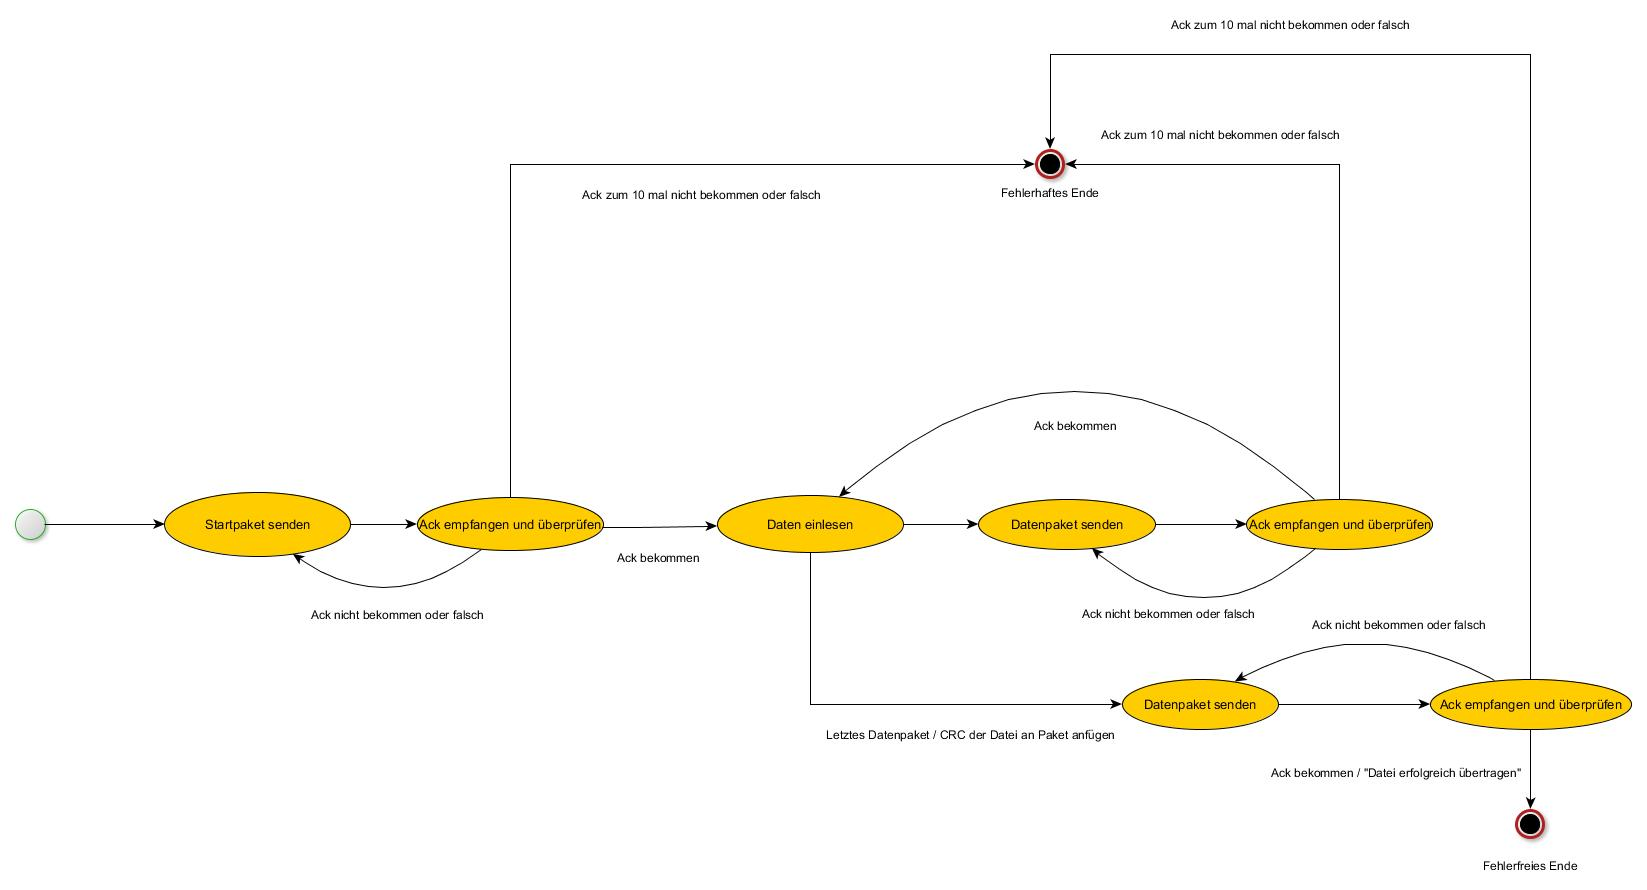
\includegraphics[height=15cm,width=24cm]{zustandsdiagram_client.jpg}
\end{landscape}
\subsection{Server}
Der Server ist zum Empfang der gesendeten Pakete zuständig und fügt nach erfolgreichem Empfangenen die Daten in einer Datei zusammen, so dass ein Abbild der vom Client(\ref{Client}) geschickten Datei auf dem Server entsteht. Dabei wird jedes erfolgreich empfangene Paket mit einen Ack bestätigt.
\subsubsection{Acknowledgement (Ack)} \label{ACK}
Mit dem Acknowledgement bestätigt der Server dem erfolgreichen Empfang eines einzelnen Pakets. Dabei enthält das Ack die Session- und Paketnummer des empfangenen Paketes  
\begin{figure}[h]
	\centering
		\begin{tabular}{|l|}
		\hline		
		\multicolumn{1}{|c|}{Acknowledgement}\\
		\hline \hline
		- Sessionnr. (2 Byte, gleiche wie im zuletzt empfangenen Paket)\\
		- Paketnr.   (1 Byte, gleiche wie im zuletzt empfangenen Paket)\\
		\hline
		\end{tabular}
\end{figure}
\subsubsection{Start des Servers}
Zum Start des Servers muss der Port angegeben werden, auf dem der Server auf eine Verbindung eines Clients warten soll.
Aufgerufen wird der Server wie der Client über ein Script:
\begin{center}
	./server-udp <Port>
\end{center}
Sollten zu wenig Parameter übergeben werden oder wird der Port schon verwendet(z.B weil Server schon gestartet wurde) kann der Server nicht gestartet werden.

\subsubsection{Programmablauf des Servers}
Nach dem Start eröffnet der Server ein UDP-Socket auf dem als Startparameter angegebenen Port.
Er fängt an auf eine Verbindung eines Clients zu warten und da im Server kein Timeout eingestellt ist, wartet der Server so lange, bis Daten empfangen werden.
\begin{javacode}
DatagramPacket receiveStartPackage =  
	new DatagramPacket(receiveStart, receiveStart.length); 
serverSocket.receive(receiveStartPackage); 
InetAddress IPAddress = receiveStartPackage.getAddress();
int port_receive = receiveStartPackage.getPort();
\end{javacode} 
Nachdem der Server ein Datagram-Paket empfangen hat extrahiert er über \textit{.getAdress()} die IP-Adresse des Clients und durch \textit{.getPort()} den Port den der Client verwendet. Der Port ist zufällig und ändert sich bei jeder Ausführung des Clients.\\\\
Ab hier läuft das Programm in einer äußeren Schleife, welche für die Daten des Startpakets zuständig ist und eine, in dieser Schleife enthaltenen inneren Schleife, welche zum Empfang der Datenpakete dient.
Folgend werden die Funktionen der Schleifen beschrieben:\\
\\
\paragraph{Äußere Schleife}

Sobald der Server das erste Paket bekommen hat konvertiert er die im Startpaket(siehe \ref{Startpaket}) enthalten Daten mit Hilfe eines Bytebuffers zurück in die Ursprungsform
\begin{javacode}
//Beispiel für die Konvertierung der Sessionnr. zurück zu einen short.
short sessionNr = startpackageBuffer.getShort(0);
\end{javacode} 
Danach überprüft der Server den CRC-Code des Startpakets indem er die Prüfsumme vom Startpaket abschneidet und dann selbst einen CRC-Code von dem restlichen Startpaket erstellt. Sind diese beiden Codes gleich wurde das Startpaket richtig empfangen.
\begin{javacode}
if (crcStartCalc != checksumStartReceived || packageNr != 0 || 
		!Kennung.equals("Start"))
{
	System.out.printf("Fehlerhaftes Startpaket.\n");
	//Warte auf neues Paket
	serverSocket.receive(receiveStartPackage); 
	IPAddress = receiveStartPackage.getAddress();
	port_receive = receiveStartPackage.getPort();
}
\end{javacode} 
Außerdem wird geprüft ob die Paketnummer wie vorgeschrieben 0 ist, und die Kennung dem String 'Start' entspricht.
Sollte eins dieser Vorgaben nicht zutreffen wird das Startpaket verworfen, und auf ein neues Paket gewartet, welches dann erneut die äußere Schleife durchläuft.\\
Sollte alles richtig sein sendet der Server ein Ack an den Client
\begin{javacode}
 ByteBuffer ACKStart = getACK(sessionNr, packageNr);
//Sende ACK
DatagramPacket sendStartACK = new DatagramPacket(ACKStart.array(), ACKStart.array().length, IPAddress, port_receive);      
serverSocket.send(sendStartACK); 
\end{javacode}
Dabei erstellt \textit{getACK()} das zu sendende Paket. Dieses wird dann über den UDP-Socket welches zum Start intialisiert wurde an den Client gesendet. 
\\
Dann überprüft der Server ob der Dateiname schon im Ordner enthalten ist.
\begin{javacode}
File file = new File(filename);
while (file.exists())
{
	String newFilename = file.getName() + "1";
	file = new File(newFilename);	
}
FileOutputStream fileOutputStream = new FileOutputStream(file);
FileChannel fileChnl = fileOutputStream.getChannel();
\end{javacode} 
Ist der Dateiname schon vorhanden wird eine '1' an den Dateinamen angefügt und erneut getestet. Dies geschieht bis ein freier Dateiname gefunden wurde.
Folgend wird ein \textit{FileOutputStream} für die Datei geöffnet. Außerdem wird ein \textit{FileChannel} geöffnet durch den in der inneren Schleife die Daten in die Datei geschrieben werden.
\\
\paragraph{Innere Schleife} Nachdem das Startpaket erfolgreich empfangen wurde und der \textit{FileChannel} geöffnet ist fängt die innere Schleife an.\\
Am Anfang dieser Schleife wird auf ein neues Paket vom Server gewartet. Wird das Paket empfangen wird aus dem Paket die Sessionnummer, die Paketnummer und, um auszuschließen, dass es kein Startpaket ist, die Kennung des Paktes ausgelesen. 
\begin{javacode}
short sessionNrData = dataPackageBuffer.getShort(0);
packageNr = dataPackageBuffer.get(2);
byte[] KennungBytesData = Arrays.copyOfRange(receiveData, 3, 8);
String KennungData = new String(KennungBytesData, StandardCharsets.US_ASCII);
	            	  
//Überprüfen ob Startpaket
if (sessionNrData != sessionNr && KennungData.equals("Start"))
{
	System.out.print("If 1\n");
	port_receive = receiveDataPackage.getPort();
	IPAddress = receiveDataPackage.getAddress();
	receiveStart = Arrays.copyOfRange(receiveData, 0, 277); 
	break;
}
\end{javacode}
Sollte sich die Sessionnr des Datenpakets von der des Startpakets unterscheiden und der String, der ausgelesen wurde der Kennung 'Start' entsprechen werden die Daten in das Bytearray des Startpakets geschrieben, die innere Schleife beendet und die äußere Schleife mit den empfangenen Daten ausgeführt.
Dann wird überprüft ob die Sessionnr. der des Startpaketes entspricht und ob die neue Paketnummer und die Paketnummer des zuvor empfangenen Pakets gleich sind (Kann z.B. vorkommen wenn Client Ack nicht bekommen hat, siehe Abbildung \ref{stop_n_wait_fail})
\begin{javacode}
if (packageNr == packageNrOld && sessionNrData == sessionNr)
{
	ByteBuffer ACKData = getACK(sessionNrData, packageNr);
	DatagramPacket sendDataACK = 
		new DatagramPacket(ACKData.array(), 
		ACKData.array().length, IPAddress, port_receive);      
	serverSocket.send(sendDataACK);     
}
\end{javacode}
Sollte dies der Fall sein werden die neu empfangenen Daten verworfen, und erneut das Ack des davor empfangenen Pakets verschickt.\\
Andernfalls werden die Daten über dem FileChanel in die Datei geschrieben, und ein Ack an den Client geschickt. Dabei wird dir Größe des Pakets zu einer Variable addiert und dann geprüft ob das letzte Paket empfangen wurde.
\begin{javacode}
receivedBytes += PACKAGESIZE;
byte[] data = new byte[PACKAGESIZE];
if (receivedBytes < fileLength)
{
	data = Arrays.copyOfRange(receiveData, 3, 3 + PACKAGESIZE);
	ByteBuffer fileDataBuffer = ByteBuffer.allocate(data.length);
	fileDataBuffer.put(data);
	fileDataBuffer.flip();
	fileChnl.write(fileDataBuffer);
	fileDataBuffer.clear();
	//Sende ACK
	ByteBuffer ACKData = getACK(sessionNrData, packageNr);
	DatagramPacket sendDataACK = new DatagramPacket(ACKData.array(),
	 		ACKData.array().length, IPAddress, port_receive);      
	serverSocket.send(sendDataACK);
	dataPackageBuffer.clear();
}
/********Falls letztes Datenpaket empfangen wird**************/
else 
{
......
if (checksumFile != checksumFileReceived )
{
System.out.print("Fehler im CRC Code der Datei..\n");
sessionNr = 0; //verhindert das für die Wiederholungspakete ein Ack gesendet wird
	            				  
}
else
{
//Sende ACK
....
\end{javacode}
Wenn das letzte Paket empfangen wird, wird die else-Anweisung ausgeführt in der, neben dem schreiben der Datei, auch der CRC-Code der empfangenen Datei erzeugt. Wenn die erstellte Prüfsumme mit der im letzen Datenpaket enthaltenen Prüfsumme übereinstimmt wird ein Ack an den Client gesendet.
Sollte sie nicht übereinstimmen wird kein Ack gesendet und durch setzen der Sessionnr. auf Null verhindert, für die Wiederholungspakete ein Ack zu senden.
\subsubsection{Bekannte Probleme}
Der Server ist nur in der Lage mit der Paketgröße des unter \ref{Client} beschriebenen Clients zu arbeiten. Um das Empfangen verschieden großer Datenpakete zu ermöglichen und dabei einen Bufferoverflow zu vermeiden müsste der Server ein Bytearray mit der Maximalgröße des UDP-Pakets (65.535 Bytes) erstellen, in dem er die empfangen Daten speichert. 
\begin{landscape}
\subsubsection{Zustandsdiagramm}
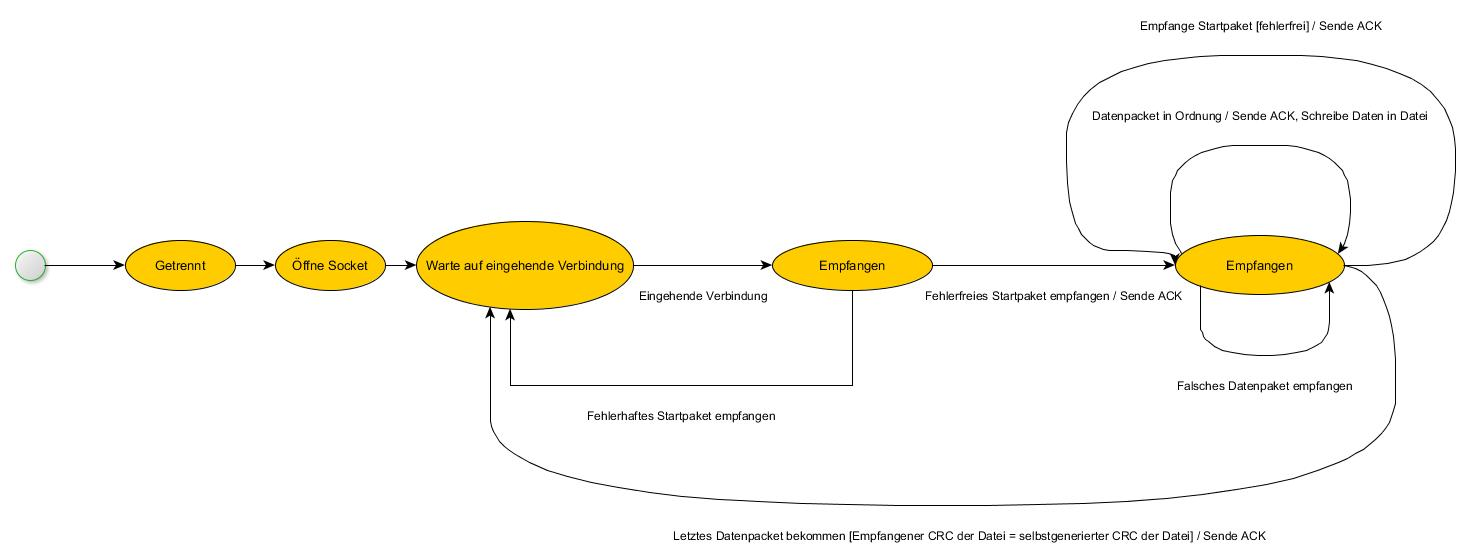
\includegraphics[scale=0.46]{zustandsdiagram_server.jpg}
\end{landscape}
\section{Verbesserungsvorschläge}
\begin{enumerate}
\item Prüfsumme für jedes Datenpaket
	\begin{itemize}
	\item Mit einer Prüfsumme am Ende jedes Datenpakets könnte man Fehler in Paketen frühzeitig erkennen. Bei Fehlern in dem CRC-Code könnte der Server sich das Paket erneut senden lassen und würde keinen falschen Daten in die Datei schreiben.
	\item Wenn die Prüfsumme erst bein letzten Paket überprüft wird muss die ganze Datei erneut gesendet werden was besonders bei größeren Dateien sehr lange dauern kann. 
	\end{itemize}
\end{enumerate}
\section*{Aufgabe 8}
\subsubsection*{Berechnung}
Bestimmung des maximalen erzielbaren Durchsatz bei 10\% Paketverlust und 10ms Verzögerung mit dem SW-Protokoll.\\
Gegeben: $P_L = 10$, $RTT = 10ms$, Packetgröße $\equiv$ L = 8192 KBit, $T_w = 10ms$,\\ 
$\text{Datenrate}\equiv r_{d} = 10^9 \text{Bit}$   \\
Berechnung: 
\begin{center}
$$\eta_{sw} = \frac{T_p}{T_p + T_w}\left(1-P_L\right)^2 * R$$
$$T_p = \frac{L}{r_b}$$
	
$$R = \frac{1024}{1024 + \underbrace{3}_{\text{Paketheader}}+\underbrace{20}_{\text{IP-Header}}}$$\newline
$$\qquad T_p = \frac{8192 + \overbrace{3\cdot8}^{\text{Größe des Paketheaders}} + \overbrace{8\cdot8}^{\text{Größe es UDP-Headers}} + \overbrace{20\cdot8}^{\text{Größe des IP-Headers}}}{\underbrace{1 \cdot 10^9}_{\text{Bei GBit-Lan}}} = 8,376 \mu s$$

$$\Rightarrow \eta_{sw} = \frac{8.376\mu s}{8.376\mu s + 10000 \mu s}\cdot(1-10)^2 \cdot R = 0,00080223 $$
$$\text{Datenübertragungsrate} \equiv r_b = \eta_{sw} \cdot r_{d} = 8,0223 \cdot 10^{-4} \cdot 10^9 = \underline{\underline{802,226 \text{KBit/s}}} $$
\end{center}
\subsubsection*{Bezug zur Praxis}
Da im Client einen Timeout benutzt und diesen bei jedem verlorenen Pakete erhöht sind die 337 KBit/s nicht zu erreichen.
\end{document}
